 %%
%%
%%   This file is based on the ``apstemplate.tex'' from
%%   the APS files in the REVTeX 4 distribution.
%%   Version 4.1r of REVTeX, August 2010
%%   See the REVTeX 4 README file for restrictions and more information.
%%
%
% This is a template for producing manuscripts for use in PHYS3605 at
% the University of Minnesota
%
% Copy this file to another name and then work on that file.
% That way, you always have this original template file to use.

\documentclass[aps,prstab,reprint,12pt]{revtex4-1}
\usepackage[title]{appendix}
\usepackage{xspace}
\usepackage{amsfonts}
\usepackage{graphicx}
\usepackage{siunitx}
\usepackage{grffile}
\usepackage{float}
\usepackage{mathrsfs}
\usepackage{physics}

\usepackage[utf8]{inputenc}

\usepackage[letterpaper, margin=0.8in]{geometry}



\providecommand{\units}[1]{\,\ensuremath{\mathrm{#1}}\xspace}


% \newcommand{\appendixpdf}[3]{
%     \includepdf[pages=1,scale=.8,pagecommand={\section{#1}\label{#3}},linktodoc=true]{#2}
%     \includepdf[pages=2-,scale=.8,pagecommand={\section*{Appendix \ref{#3}\quad #1}},linktodoc=true]{#2}
% }

% \linespread{2}

\begin{document}

%Title of paper
\title{A Relation of Mechanical and Electrical Power using a Watt Balance}

% Your name should go first, marked as ``communicating author'' 
\author{M. Laraia and J. Hirschi}
% Your lab partner or partners can come next

\affiliation{University of Minnesota, Minneapolis, MN, USA}

\date{\today}

\begin{abstract}
A Watt balance is constructed to measure the relationship between mechanical power and electrical power. The flux through the measurement coil was measured by statically balancing the weight of an object, and while oscillating the balance arm. These two measurements yielded values that were proportional to $0.98 \pm 0.11$.
\end{abstract}

\maketitle

\section{INTRODUCTION}

The International System of units (SI) is being redefined in 2019. In the original system, some of the units were defined in terms of physical objects. The Kilogram, for example, was defined by the International Prototype Kilogram (IPK). The IPK is a block of platinum-iridium alloy forged in 1879 and stored underground in Paris ever since, together with a number of identical sister copies. Every scientific measurement of SI mass is relative to the mass of the IPK. It has been shown, however, that the mass of the IPK and its sister copies has been diverging over time, as shown in figure~\ref{fig:ipk_divergence}. Defining a unit in terms of a physical object is problematic as it cannot be guaranteed that the properties of the object will remain static over long time periods.

For this reason the SI system of units is being redefined to rely only on fundamental constants of the universe. As an example, the meter can be defined in terms of the speed of light in vacuum, and the second can be defined in terms of the frequency of light emitted in a specific energy transition in Caesium-133.
The Kilogram can be defined in terms of Planck's constant, and a device that can measure this relationship is a Watt balance.

% Maybe reword, be more concise but still conveying the story
% Maybe the first figure should be the mass drift figure?

%\begin{figure}[h]
    %\centering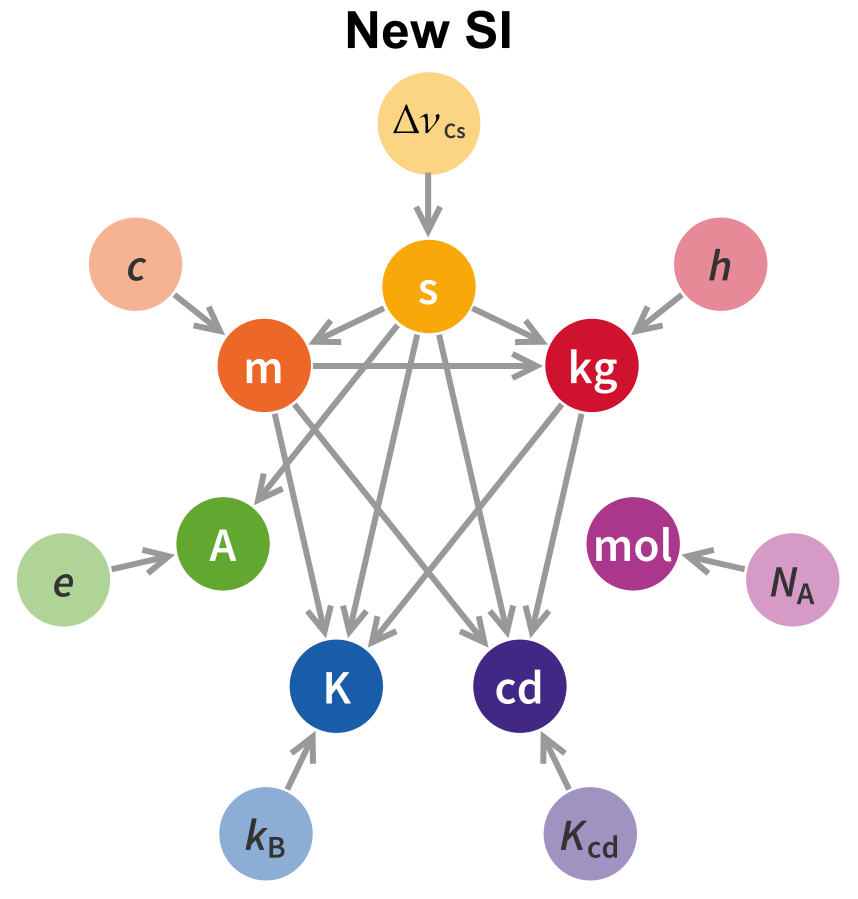
\includegraphics[width=.95\linewidth]{figs/si_units.png}
    %\caption{As of May 20, 2019, all SI units will be defined in terms of fundamental constants of the universe. 
    %\cite{wiki_si}}\label{fig:si}
%\end{figure}

\begin{figure}[t]
    \centering
    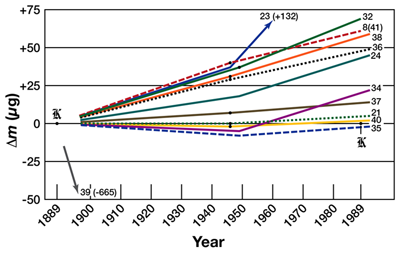
\includegraphics[width=0.95\linewidth]{figs/ipk_mass_drift.png}
    \caption{The mass of the IPK and its sister copies. Evidently the mass of the IPK is diverging from the mass of the copies over time.}
    \label{fig:ipk_divergence}
\end{figure}

%For this reason there is a push to redefine the SI units in terms of fundamental constants of the universe, as many of the original SI units were defined in a similar and sometimes arbitrary way. For example, length has been redefined in terms of speed of light in vacuum, and time in terms of the period of radiation of a specific transition in caesium-133. The kilogram, ampere, kelvin, and mole are the last remaining SI units to be redefined in such terms. A summary of the fundamental dependencies of the redefined SI system is shown in figure \ref{fig:si}. 
%Additional discussion of redefinition

%After the SI system has been defined in terms of fundamental constants of the universe, anybody anywhere will be able to measure a unit in the SI system. This means that an instrument need not be calibrated to a standard object, like the IPK, but instead can be calibrated directly by measuring the fundamental constants. This guarantees that our system of measurements will remain constant through time, and furthermore ensures the repeatability of any physical experiment far into the future.


What follows is a general description of how a Watt balance works. A more detailed description will follow in sections~\ref{s:theory} and~\ref{s:device}.
A watt balance resembles an equal arm balance with each side of the arm having a permanent magnet hanging over coiled wire. The Watt balance is operated in two modes. In the first mode an object is placed on the balance, and a current applied to one coil creates a force on the adjacent permanent magnet that acts against the weight of the object. In the second mode one of the coils is driven to oscillate the balance arm. The motion of the permanent magnet in the second coil induces an electromotive force that can be measured. The two modes are called the force mode and the velocity mode.


%A watt balance is effectively an equal arm balance where the weight of an object acts against an electromagnetic force. More generally, a watt balance balances mechanical power with electrical power. The electromagnetic force in this situations is the force acting on a magnetic quadrupole near a current carrying loop of wire. A watt balance that can generate precise electrical power to balance the mechanical power acting on the object can therefore be used to directly measure the mass of the object. What remains is linking the electrical power to Planck's constant.

Planck's constant can be recovered when measuring induced emf in the velocity mode and the applied current in the velocity mode. The induced emf can be measured with Josephson junctions, and the applied current in the force mode can be measured with a Josephson junction measuring the voltage over a quantum Hall resistance standard. This is discussed further at the end of section~\ref{s:theory}.

%Planck's constant appears when considering the Josephson effect and the Hall effect of quantum mechanics. The Josephson effect provides a quantized voltage standard, and the quantum Hall effect provides a quantized resistance standard, both of which relating Planck's constant to the frequency of an applied electromagnetic wave. Together these quantum effects can be used to measure electrical power, and a Watt balance utilizing these effects can directly relate the mass of the object to Planck's constant. We discuss this further at the end of section \ref{s:theory}


The official Watt balance at the National Institute of Standards and Technology was built with Josephson junctions and quantum Hall resistance standards. To redefine the SI kilogram, the Watt balance was used with a standard mass calibrated to the IPK to fix Planck's constant relative to the kilogram. After redefinition, a Watt balance could be used to precisely measure the mass of a standard mass in terms of Planck's constant.

%The National Institute of Standards and Technology (NIST) constructed a Watt Balance utilizing these quantum effects. The measurements from this device are used to fix Planck's constant in terms of the IPK. After redefinition, a Watt balance utilizing the quantum effects can be used to measure the mass of an object in terms of Planck's constant.

This provides the motivation for building a Watt balance. As we do not have access to Josephson junctions and quantum Hall resistance standards for this experiment, the device and the experiment described here will not measure the relationship to Planck's constant. Instead we aim to build a Watt balance that can relate the mechanical and electrical power in the two modes described above.
%The device we build in our experiment will not be able to rely on the Josephson effect and quantum Hall effect in our measurements, as utilizing these effects would each constitute semester projects on their own. Therefore we do not expect to be able to relate our measurements to Planck's constant. Instead the focus of our experiment will be to construct a device capable of balancing mechanical power with electrical power in the style of a Watt balance described above with the two modes of operation. We hope that our work in constructing such a device can be extended by other groups in the future to measure Planck's constant by using the Josephson and quantum Hall effects.


\begin{figure}
    \centering
    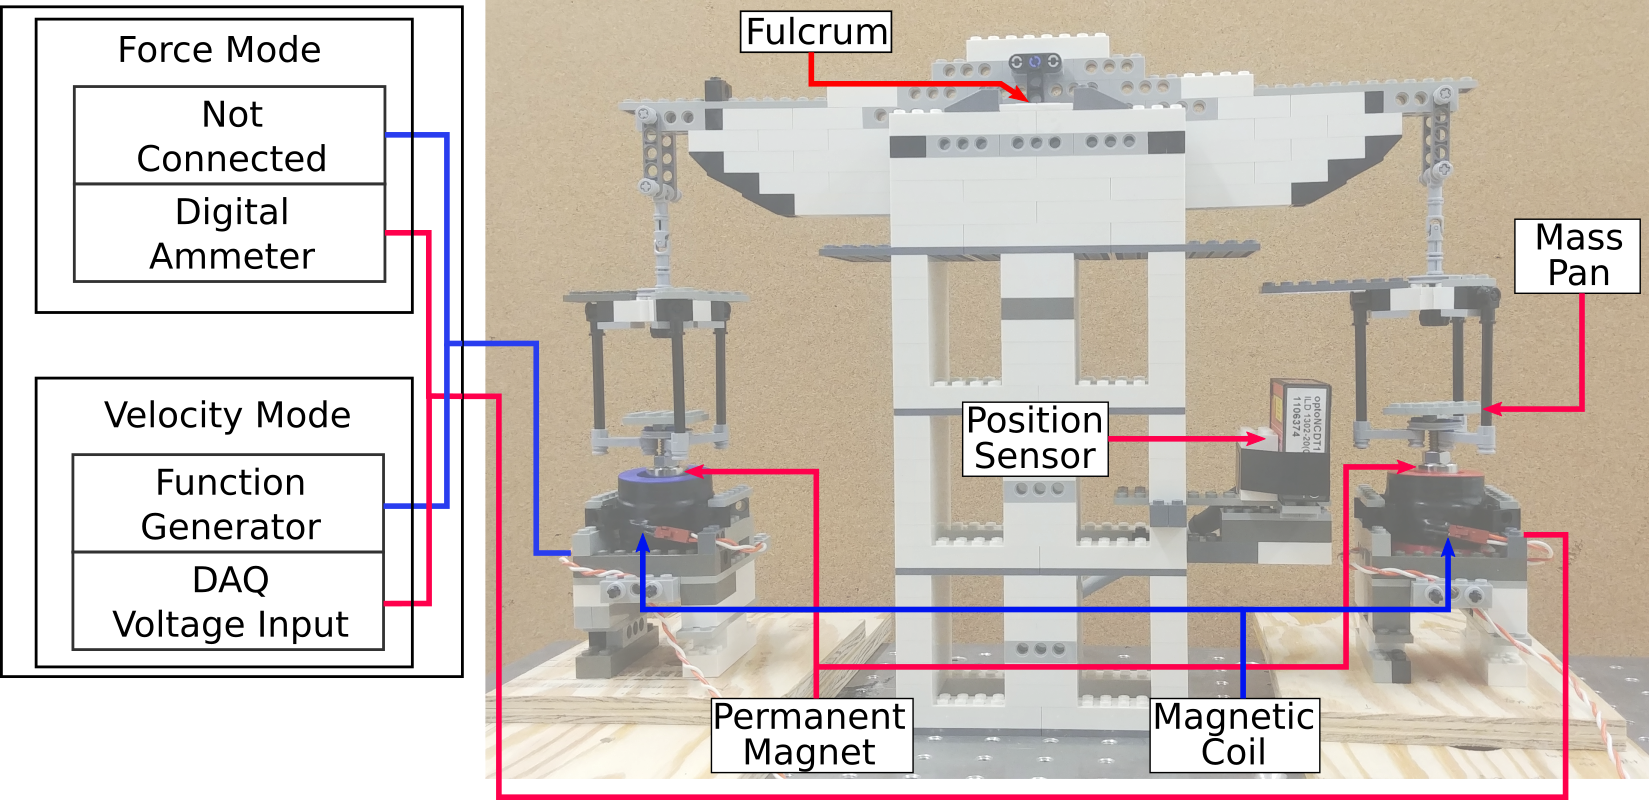
\includegraphics[width=0.95\linewidth]{figs/watt_balance.png}
    \caption{TODO}
    \label{fig:device_image}
\end{figure}


\section{THEORY}\label{s:theory}

A Watt balance operates by balancing an electromagnetic force with a mechanical force. This can be done by operating the Watt balance in two modes. In the velocity mode one coil is driven to create oscillating motion in the arm while the other coil uses Faradays law to measure an induced electro-motive force $\mathscr{E}$. In the force mode only one coil is operated to provide a force which balances the gravitational force acting on a mass. As mentioned earlier, the velocity mode is a pseudo-calibration step, which will be described in further detail in this section.

Faraday's Law states that when a permanent magnet moves near a looped wire, an emf $\mathscr{E}$ is produced, which induces a voltage in the wire proportional to the number of loops $N$ and the rate of change of the magnetic flux $\Phi_B$
\begin{equation}\label{eq:Faraday}
\mathscr{E} =-N\frac{d \Phi_B^N}{dt}.
\end{equation}

If we assume that the rate of change of the magnetic flux is proportional to the velocity of the permanent magnet, then we can rewrite this equation as follows, where $\Phi_v = (\Phi_B^NN)_v$:
\begin{equation}\label{eq:velocity_equation}
    \Phi_v  = \frac{V}{v}
\end{equation}

When the balance arm is driven in the velocity mode, a voltage is induced proportional to the magnetic flux $\Phi_v$ and the velocity of the arm. This measurement can be used to factor out the flux $\Phi_f$ in the force mode, as will be described below.

The Lorentz force law can be described as follows, where $q$ is a charge, $v$ is its velocity, $E$ is the electric field, and $B$ is the magnetic field:
\begin{equation}
    \vec{F} = q(\vec{E}+v\times \vec{B})
\end{equation}

We can drop the electric field term because the latent electric field is negligible compared to the magnetic field. Expressing the second term in terms of the current $I$ through a length of wire $l$ yields the following:
\begin{equation}
    \vec{F} = I \vec{l}\times \vec{B}
\end{equation}

If the wire is instead looped, then we can integrate this equation over the length of the loop as follows to get a force in the direction normal to the plane of the loop $\hat{n}$:
\begin{equation}
    \vec{F} = I\int\vec{dl}\times\vec{B}  = (\Phi_B^N N)_fI \hat{n}
\end{equation}

In the force mode the Watt balance will be operated to generate a force counteracting the gravitational force on a mass $m$. This produces the following relationship, where $\Phi_f = (\Phi_B^NN)_f$
\begin{equation}\label{eq:force_equation}
    \Phi_f = \frac{mg}{I}
\end{equation}
where $g$ is the local acceleration due to gravity. The two modes of measurement and their force diagrams are illustrated in figure~\ref{fig:Force}. 

\begin{figure}[t]
     \centering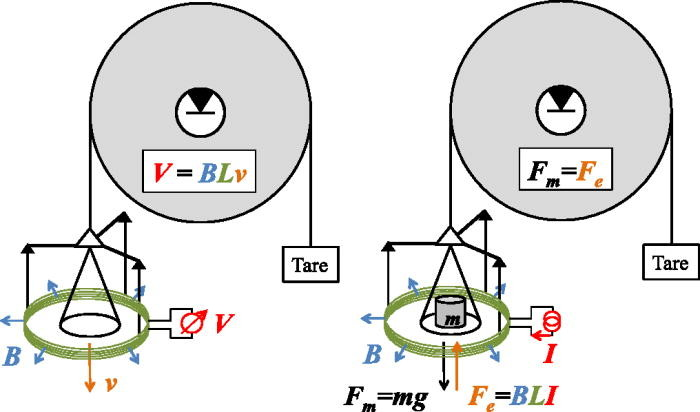
\includegraphics[width=.95\linewidth]{figs/Force_Diagram.jpeg}
     \caption{Velocity mode measurement, illustrated on the left, depicts a coil moving vertically in a radial magnetic field and a voltage $V$ is induced. Force mode measurement, right, displays that the upward electromagnetic force generated by the coil opposes the gravitational force exerted on the mass. \cite{Chao2015}}\label{fig:Force}
\end{figure}

\begin{figure}[t]
    \centering
    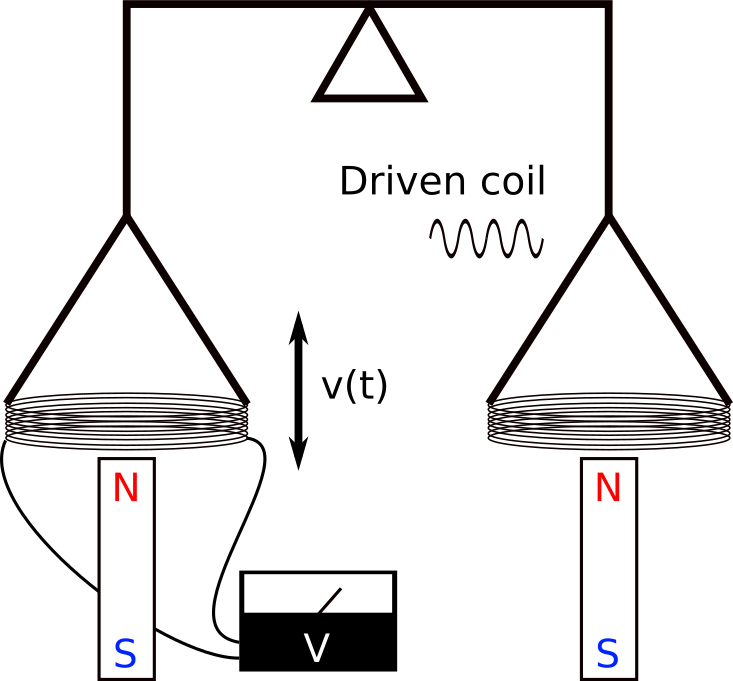
\includegraphics[width=0.6\linewidth]{figs/watt-balance-vmode.png}
    \caption{Velocity mode concept  TODO}
    % TODO
    \label{fig:vmode-concept}
\end{figure}

\begin{figure}[t]
    \centering
    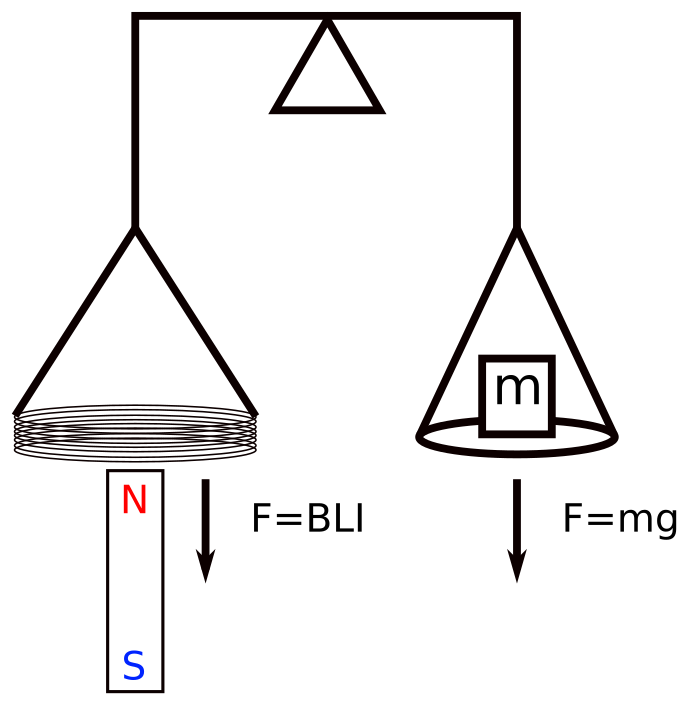
\includegraphics[width=0.6\linewidth]{figs/watt-balance-fmode.png}
    \caption{Force mode concept TODO}
    % TODO
    \label{fig:fmode-concept}
\end{figure}

Assuming that $\Phi$ remains constant between measurements in the velocity and force modes, equations~\ref{eq:velocity_equation} and~\ref{eq:force_equation} can be used to factor out the $\Phi$ term. This is important because the flux $\Phi$ is very difficult to measure directly. Furthermore, any linear correction factors that would normally have to be considered in such a setup can be accounted for in the same way as $\Phi$. We expect these factors to be present and equal in both modes of operation and can therefore be rolled in with $\Phi$. Possible linear correction factors of this sort include the moment of inertia of the balance arm and various linear sources of friction. We arrive at the following equation
\begin{equation}\label{eq:watt_equation}
    \frac{\Phi_f}{\Phi_v} = \frac{VI}{mgv} = 1
\end{equation}

Equation~\ref{eq:watt_equation} relates mechanical power $mgv$ to electrical power $VI$. In our experiment we will measure $V$, $I$, and $v$, assuming $m$ and $g$ are known.

A successful experiment would measure a 1-to-1 correspondence between electrical and mechanical power, confirming equation~\ref{eq:watt_equation}. If successful, the watt balance we build could be used to measure other quantities. For example, if the mass of an object is known equation~\ref{eq:watt_equation} can be used to measure the local gravitational acceleration. Conversely, if the local gravity is known we can measure the mass of an unknown object.

Finally, we provide an additional discussion on the quantum effects used in the official NIST Watt balance. 
The Josephson effect is an effect in the quantum realm describing current across a Josephson function. A Josephson junction consists of two superconductors coupled by a weak link.\ 
when an electric field oscillating at a microwave frequency $f$ is applied a small current is forced through the junction. This creates a quantized voltage across the junction.
Many Josephson junctions can be combined to create a voltage standard that couples the generated voltage to Planck's constant as follows, where $h$ is Planck's constant, $e$ is the charge of an electron, and $K_J$ is Josephson constant
\begin{equation}\label{eq:josephson}
    V=\frac{h}{2e}f \equiv \frac{1}{K_J} f
\end{equation}
The NIST Watt balance uses 250,000 junctions to measure any voltage up to 10\si{V} with a precision of 1\si{nV}. The approximate \$100,000 cost of this setup makes it unfeasable in an MXP classroom setting \cite{Chao2015}.

The quantum Hall effect is a special case of the classical Hall effect, but where the Hall conductance is quantized. This effect occurs in two-dimensional systems of electrons subjected to low temperatures and strong magnetic fields. The quantized Hall conductance $\sigma$ can be described as follows, where $\nu$ belongs to either the set of integers or to a set of known fractions
\begin{equation}
    \sigma = \frac{I}{V_\mathrm{Hall}} = \nu \frac{e^2}{h}
\end{equation}

If we consider only the integer Hall conductance, then we arrive at the following quantized Hall resistance $R_H$, where $R_K$ is the von Klitzing constant
\begin{equation}\label{eq:resistance}
    R_H=\frac{V_H}{I}=\frac{1}{\nu}\frac{h}{e^2} \equiv \frac{1}{\nu} R_K
\end{equation}

The NIST Watt balance uses the quantum Hall effect to measure resistance with a relative uncertainty of 1 in $10^9$. Together with a Josephson voltage standard this can be used to measure current with incredible precision. To determine the value of $VI$ from equation~\ref{eq:watt_equation}, we combine two Josephson standards from equation~\ref{eq:josephson} and a Hall resistance standard from equation~\ref{eq:resistance} to yield the following expression, where $C$ is a known constant related to the number of Josephson junctions
\begin{equation}
    VI=V \frac{V_H}{R_H} = C f_1 f_2 \left(\frac{h}{2e}\right)^2 \frac{e^2}{h}=C \frac{f_1f_2}{4} h
\end{equation}

We see that $h$ finally drops out, and plugging back into equation~\ref{eq:watt_equation} yields the following expression
\begin{equation}\label{eq:planck}
    C \frac{f_1f_2}{4} h = mgv
\end{equation}

Equation~\ref{eq:planck} defines the kilogram in terms of Planck's constant and other measurements in units defined by other fundamental constants of the universe. This is the desired result.




%%%%%%%%%%%%%%%%%%%%%%%%%%%%%%%%%%%%%%%%%%%%%%%%%%%%%%
%%%%%%%%%%%%%%%%%%%%%%%%%%%%%%%%%%%%%%%%%%%%%%%%%%%%%%
\section{EXPERIMENTAL SETUP} \label{s:device} %%%%%%%%
%%%%%%%%%%%%%%%%%%%%%%%%%%%%%%%%%%%%%%%%%%%%%%%%%%%%%%
%%%%%%%%%%%%%%%%%%%%%%%%%%%%%%%%%%%%%%%%%%%%%%%%%%%%%%

\begin{figure}[t]
    \centering
    \includegraphics{figs/device-diagram.png}
    \caption{Device diagram TODO}
    \label{fig:device_diagram}
\end{figure}


In this section we describe the device construction. An image of the completed design is shown above in figure~\ref{fig:device_image}. A diagram of the experimental setup is shown in figure~\ref{fig:device_diagram}.
LEGO bricks were chosen to build this device as it is easy not only to quickly build a prototype, but also to make modifications to the prototype along the way. An arm balances on a central tower.
From each end of the arm hangs a platform. A universal joint is used to hang the platform from the arm to allow the platform to hang freely. From each platform hang a pair of permanent neodymium magnets.
The magnets are oriented antiparallel in a quadrupolar configuration. Below each pair of magnets is a 3D-printed cylinder that carries the coiled wire.
The cylinder is designed with a groove to hold the wire. 3,000 turns of 36-AWG magnetic wire are wound onto each cylinder.

The two coils are labeled as the red coil and the blue coil to limit confusion. In the velocity mode, the blue coil is connected to an HP Agilent 33120A arbitrary waveform generator (function generator). The red coil is connected to an NI 6321 data acquisition (DAQ) card to measure the induced voltage. In the force mode the blue coil is disconnected. The red coil is connected in series to an SRS600 low noise preamplifier and an HP 34410A digital multimeter configured to measure current. The SRS600 output is controlled by the DAQ card.

A previous design had the permanent magnets mounted on the base and the coils suspended from the platforms. The configuration described here has the coils mounted on the base and the magnets suspended from the platforms. This configuration was chosen as the wires to the coils suspended from the platform were too rigid to allow the platform to hang freely as the arm moved. The drawback to the configuration with the suspended magnets is that as each magnet weights % TODO magnet weight
, the moment of inertia of the arm is increased significantly.


A MicroEpsilon laser triangulation displacement sensor is mounted below one of the platforms. This sensor is sensitive to within 1\si{\mu m} within a measurement range of 30-50\si{mm}. The top of the platform stage is extended with a flat LEGO brick to reflect the displacement sensor laser. A piece of white printer paper is attached below this extension to ensure the shape of the LEGO brick does not distort the reflection of the laser. The displacement sensor is connected to the measurement computer with an RS232 serial interface.


% 
% In this section we describe the construction of the Watt balance. The design is based on the Lego Watt balance design illustrated in \cite{Chao2015}, but with some modifications which will be explained below. An image of the completed design is shown in figure \ref{fig:our_balance}.
% 
% The design resembles that of a traditional equal arm balance: there is an arm balancing on a small fulcrum with two pans hanging on either side. The pans hang from the balance arm with a universal joint to allow the pans to hang freely. From each pan hangs a brass screw with two neodymium ring magnets mounted. The magnets are oriented such that the magnetic dipoles are aligned anti-parallel. Beneath each magnet pair there is a coil of wire. The coils are 3,000 turns of 36-AWG wire wound around plastic 3D-printed cylinders. The coils are positioned below the magnets with about 10\si{mm} clearance. Increasing the clearance lifts the magnets out of the coils. This gives the balance arm a larger range of motion, but will decrease the magnitude of the magnetic flux through the coils.
% 
% Both the force mode and velocity mode require knowing the displacement of the magnets from the balanced position. For this purpose a compact laser triangulation displacement sensor, specifically a Micro-Epsilon optoNCDT ILD1302, is used. This sensor has a measurement range of 30mm to 50mm. 
% % TODO resolution of micro epsilon?
% The sensor is attached to the base of the device and oriented to point at a bar extending from one of the pans. The device is positioned so the range of motion of the arm falls within the measurement range of the device. The device determines the position of the arm by reflecting a laser off the bar. A smooth piece of paper is glued to the bottom of the bar to ensure the laser reflects uniformly from the surface.
% 
% One coil is connected to an HP Agiletn 33120A function generator, which is controlled by a LabView program. This coils is only driven in the velocity mode. The other coil is connected to two different devices depending on the mode of operation. In the velocity mode we measure the current through the coil, while in the force mode the coil is driven with a steady current. In both modes this coil is connected to a data acquisition card (DAQ).
% % TODO determine what daq card we're using
% To protect the DAQ from the large load of the coil an amplifier is connected between the DAQ and the coil for the force mode.
% % TODO determine what amplifier we are using
% 
% % TODO explain why the coils are positioned below instead of above
% Previous work in building a Lego based Watt balance \cite{Chao2015} had the permanent magnets mounted below with the coils hanging from the pans. Such a design would have wires running from the coils up past the pans to the arm, then to the center of the arm, then down through the center of the base. We found that these wires were stiff enough to apply a torque at two locations. Both the balance of the arm as well as the balance of the pans below the arm were affected. We instead decided to hang the permanent magnets from the pans and place the coils on the ground. The permanent magnets are significantly heavier than the coils, so such a configuration significantly increases the moment of inertia of the balance. 
% % TODO do we need to add a sentence at the end of this? To say why it's ok to swap the magnets and the coils




\section{PROCEDURE}


In this section we describe the data acquisition process. In the first stage the emf induced in the loop is measured as a function of the velocity of the balance arm. In the second stage the current required to balance the arm is measured for a given mass configuration. We begin by describing the data acquisition process for the velocity mode. % definitely need a TODO

The displacement data is gathered from the MicroEpsilon displacement sensor with a LabView program. The LabView program runs at a fixed 100Hz frequency, while the measurement rate of the displacement sensor is 750Hz \cite{muepsilon_sheet}. To compensate for this difference the measurements collected at each time step are averaged. An added benefit is that this smooths the noisy signal from the displacement sensor.

\subsection{VELOCITY MODE}

In the velocity mode the blue coil is driven with the function generator while the induced voltage in the red coil is measured with the DAQ. The function generator used in this experiment has a lower signal amplitude limit of 50\si{mV_{pp}}. To further reduce the signal amplitude the red coil is separated from the function generator output with a 1:10 voltage divider circuit.

During a measurement run the function generator was configured to output a signal with an amplitude range of $50-300$ \si{mV_{pp}} and a frequency range of $100-1000$ \si{mHz}. This frequency range was chosen to be close to the natural frequency of the balance arm, which was determined to be roughly in the range $550-650$ \si{mHz}. The signal amplitude for a particular measurement run and frequency were chosen such that the measured peak-to-peak displacement was approximately 1\si{mm}. The LabView program was configured to collect data with a 10ms time step.



%A LabView program collects time series measurements of the magnet displacement and induced voltage in the red coil.

%Both coils are used in the velocity mode measurement. In this section Coil A refers to the coil where the induced emf is measured, while Coil B refers to the coil being driven. Coil B is driven by the function generator with a sinusoidal wave with frequency $500\si{mHz}$ and amplitude $0.5V_{pp}$. The natural frequency of the balance arm was found to be near 650mHz. The coil is driven near the natural frequency but not quite at the same value.
%% TODO why^

%Driving Coil B oscillates the permanent magnets in and out of coil A. This induces an emf in coil A proportional and in phase with the velocity of the oscillatory motion. While Coil B is driven, the micro-epsilon sensor measures the position of the bar over time while the DAQ measures the amplitude of the induced emf over time. The LabView program running the data acquisition program ensures that the position and emf measurements are synchronized to within a few milliseconds. A time step of $10\si{ms}$ is used for both measurements. The velocity is determined from the position data by calculating the symmetric difference quotient of the position data with respect to time. The constant of proportionality between the velocity $v$ and emf $\mathscr{E}$ gives the desired quantity of the magnetic flux $\Phi_B N$. This can be determined from the measurements using a linear least squares regression.


\subsection{FORCE MODE}

In the force mode a current is applied to the red coil to oppose the weight of a mass placed in the mass pan. A LabView program controls the current output to the red coil using a PID controller. A PID controller is a control-loop feedback mechanism to continuously modulate an output to move the system to a desired state.
The PID calculates the error between the desired input (setpoint) and the measured process variable.
The PID calculates a correction with three terms, the proportional, the integral, and the differential terms. At each time step the proportional term considers the current value of the error, the integral term considers how long the error has persisted, and the differential term considers how the error changes over time.
More information about PID theory can be found in \cite{pid}.

The magnitude of the proportional, integral, and differential corrections is determined by the paramters $K_p$, $K_I$, and $K_d$. The values for these constants were determined through trial and error. The PID was run with an arbitrary mass on the balance.
The parameters were tuned first by adjusting $K_p$ and $K_I$ until the balance was able to slowly bring the process variable near the set point.
Then the $K_d$ term was increased until the PID was able to counter small oscillations about the set point. The parameters were accepted when the balance was able to go start from rest and remain within 1\% of the setpoint for more than 5 seconds. The values for the parameters are summarized in table~\ref{tab:pid}. The setpoint was determined by placing a level over the center of the balancing arm and varying the setpoint until the balance arm was level. Using this method the setpoint was chosen as 8.5mm.

\begin{table}
    \centering
    \begin{tabular}{|c|c|c|}\hline
        $K_p$ & $K_I$ & $K_d$ \\\hline
        0.1 & 0.01 & 0.005 \\\hline
    \end{tabular}
    \caption{Tuned parameters for the PID controller. These parameters are used to operate the Watt balance for the force mode measurement.}
    \label{tab:pid}
\end{table}

Two current measurements are made when making a force mode measurement. In the first step the current required to balance a tare mass is recorded. The mass of the tare mass does not need to be known, as will be shown in a moment. In the second step a known mass is placed on the opposite coil, and the current required to balance both masses is recorded. 
\begin{align}
    I_T \Phi_f &= -m_T g ,\quad I \Phi_f = (m-m_T)g \nonumber \\
    \Phi_f &= \frac{mg}{I-I_T} \label{eq:force_current}
\end{align}
As equation~\ref{eq:force_current} shows, the tare mass is irrelevant. It is possible that the current required to balance the mass will drift. To correct for the drift these steps are repeated 2-3 times for a given measurement run. The resulting measurements with and without the mass are averaged to get $I_T$ and $I$.

The mass of a given object was determined with a chemical scale accurate to 1mg. The mass was varied in small increments by bundling small amounts of wire. The tare mass used was typically a 2g calibrated mass. The resulting measurements are shown in figure!\ref{fig:both-data}, and will be discussed further in section~\ref{s:discussion}.

%This measurement involves placing a known mass onto the mass pan, located above coil A in figure \ref{fig:chao_balance}, and inducing an electromagnetic force on coil B to counteract the gravitational force of the mass. The magnitude of the electromagnetic force will be controlled in a way such that the balance arm will stay in it's nulled position after masses are added or removed. A proportional integral derivative controller (PID), programmed using LabVIEW, will be used to regulate the electromagnetic force. This type of controller uses manual feedback to automate the changes necessary in the
%electromagnetic force to hold the balance in the null position. Several constants will need to be determined and inputted into the PID controller to regulate this specific system.

%The measurement process will involve measuring the current needed to balance a tare mass and a calibrated mass. We can then relate the two measurements to solve for the $(\Phi_B N)_F$ factor. However, to cancel out any drift that may occur in our measurements of current the measurement process will be repeated multiple times with the same masses. This will improve the accuracy of calculated $(\Phi_B N)_F$ factor. In order to calculate the flux integral from force mode, we need to know the local gravitational constant $g$ which can be referenced from the National Oceanic and Atmospheric Administration.

% \subsection{Relation of Mechanical and Electrical Power}

% If successful, our watt balance will measure a 1-to-1 correspondence between $(\Phi_B N)_v$ and $(\Phi_B N)_F$. 


\section{DATA ANALYSIS}\label{s:discussion}

In this section we describe the steps used to process and analyze the measured data. The general formula for propagasub
The error propagation for a multi-variable function $\gamma$ defined for $n$ variables $\delta_1\cdots\delta_n$ is defined as follows
\begin{equation}
    \sigma_\gamma^2 = \sum_{\delta_1}^{\delta_n} \sigma_\delta^2 \left( \frac{\partial \gamma}{\partial \delta} \right)^2
\end{equation}
All uncertainties quoted in this analysis are calculated using this formula.

For the force mode we made at least two measurements each of $I_T$ and $I$. We calculate each current as the mean of these measurements, and the uncertainty as the sample standard deviation. If the standard deviation is less than 0.01mA then this value is used instead.

The resulting force measurements are shown in figure~\ref{fig:both-data}a. A linear least squares regression was performed on the mass vs current data. The reduced $\chi^2$ value for the fit was 1.35, which suggests the fit is good.

The local gravity can be estimated using a tool provided by the National Oceanic and Atmospheric Administration (NOAA) for a given geographic location. Using this tool and the coordinates of the lab (44.975224 N, 93.234298 W, 830ft above sea level) the local gravity is estimated as $g=980585\pm2\mathrm{milligal}$. Using equation~\ref{eq:force_current} the factor $\Phi_f$ can be extracted from the slope of figure~\ref{fig:both-data}a and this value for gravity. The value of $\Phi_f$ is determined to be $25.55 \pm 0.51\si{\frac{kgm}{s^2A}}$


Calculating the $\Phi_v$ term for the velocity mode has a few additional steps. The first problem arises when trying to calculate the time derivative of the displacement data. One method to calculate the derivative of a signal is the centered difference method (CD), a variation of the finite difference \cite{finite_diff}.
The central difference is defined as
\begin{equation}
    f'(x) = \frac{f(x+h)-f(x-h)}{2h}
    \label{eq:diff}
\end{equation}
Figure~\ref{fig:savgol} shows in blue a sample of velocity calculated using the central difference method.
The noise that is present in the original displacement data is significantly amplified when calculating the derivative.
To suppress this noise we use a Savitzky-Golay (SG) filter to smooth the displacement data before calculating the derivative.
An SG filter works by fitting an n-th order polynomial to a window of the data, and slides the window across the data set.
More detail on the SG filter can be found in \cite{press1990savitzky}.
The results of calculating the velocity on the sample data using a SG filter with a window size of 51 and fitting to a 3rd order polynomial are shown in yellow figure~\ref{fig:savgol}.
As the figure shows the velocity calculation using the SG method agrees well with the velocity calculated using the CD method with significant noise suppression.

\begin{figure}[t]
    \centering
    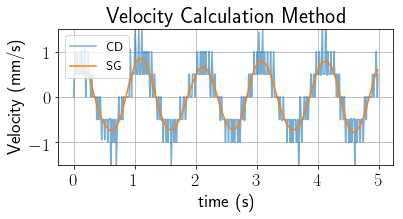
\includegraphics[width=\linewidth]{figs/data/velocity_savgol.png}
    \caption{TODO}
    \label{fig:savgol}
\end{figure}

An example of standardized time series voltage and displacement measurements for a measurement run are shown in figure~\ref{fig:correlation}a. The figure demonstrates that the velocity data lags behind the voltage data. The amount of lag can be determined using cross-correlation, which put simply is the sliding inner product of the two series. Cross-correlation is explained further in appendix~\ref{apx:correlation}.
This time lag is determined to be 120ms in every measurement run conducted for this experiment, with a few outliers at 110ms or 130ms. These measurement runs were conducted with different frequencies, signal amplitudes, and average displacement of the magnet in the coil.
Furthermore it is nonsensical to expect the induced voltage to lead the motion of the magnet. These two points suggest that the time lag is not physical, and is instead a systematic in the data collection process.

\begin{figure}[t]
    \centering
    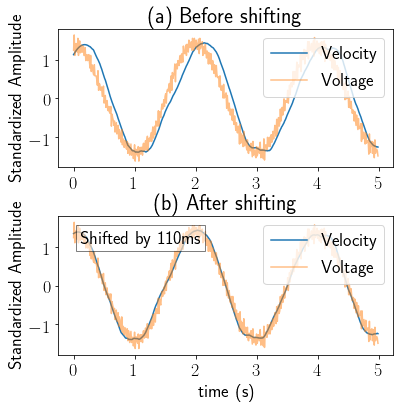
\includegraphics[width=\linewidth]{figs/data/autocorrelation.png}
    \caption{TODO}
    \label{fig:correlation}
\end{figure}

One possible explanation is that the RS232 serial interface between the displacement sensor and the LabView program has some fixed overhead that could be contributing to the lag.
Another possible explanation is that the LabView program itself is contributing to the lag in the way it collects the data, averages it, and assigns it to a specific time step.
Further inquiry is needed to determine the exact source of the time shift.

An example of the induced voltage and velocity of a measurement run in the velocity mode is shown in figure~\ref{fig:velocity-example}. The data in this figure was prepared using the methods described above. For clarity only a 250 point random sample of the full measurement run are shown. The reduced $\chi^2$ value of the fit is 4.21, suggesting the fit is reasonable but some of the uncertainties may be underestimated. The factor $\Phi_v$ can be determined from the slope of this figure using equation~\ref{eq:velocity_equation}. The $\Phi_v$ factor for this example is determined to be $27.325 \pm 0.077\si{Vs/m}$

\begin{figure}[t]
    \centering
    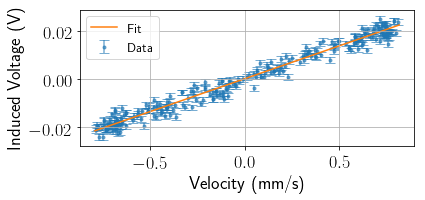
\includegraphics[width=0.95\linewidth]{figs/data/velocity_data_example.png}
    \caption{TODO}
    \label{fig:velocity-example}
\end{figure}

The PID setpoint for the force mode measurements was 8.5mm. The center about which the magnets oscillate in the velocity mode can be varied by adding a tare mass to the balance. This experiment assumes that the magnetic field created by the magnets is approximately uniform for small perturbations in the velocity mode. However, as the permanent magnets form a quadrupole, the magnetic field does vary depending on the displacement of the magnets.

\begin{figure}[t]
    \centering
    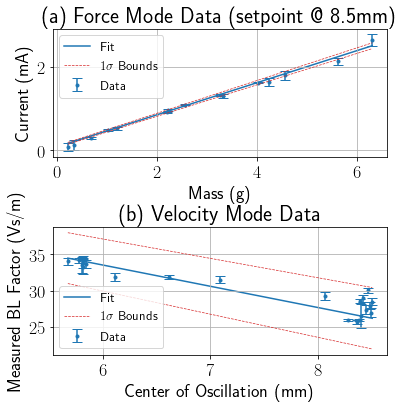
\includegraphics[width=\linewidth]{figs/data/final_data.png}
    \caption{TODO}
    \label{fig:both-data}
\end{figure}

The relationship between $\Phi_v$ and the center of oscillation can be determined by varying the center of oscillation and using the above described method to measure $\Phi_v$. This model can then be used to predict the value of $\Phi_v$ when the balance is oscillating about the 8.5mm displacement used as the setpoint in the force mode measurements. These measurements are shown in figure~\ref{fig:both-data}b. The model predicts a value for $\Phi_v$ as $26.2 \pm 3.0$\si{Vs/m}. The value for $\Phi_v$ differs from $\Phi_f$ by $0.2\sigma$. The error rate of the measurements can be defined as $(\Phi_v-\Phi_f)/\Phi_v$. The error rate for these measurements is 2.4\%.

The goal of this experiment was to measure unity between $\Phi_f$ and $\Phi_v$, as expressed in equation~\ref{eq:watt_equation}. The measurements described above yields a value for $\Phi_f/\Phi_v$ of $0.98 \pm 0.11$. Unity is within the margin of error for this value, suggesting the experiment was successful. 




%\section{DISCUSSION}




%\begin{figure}[t]
    %\centering
    %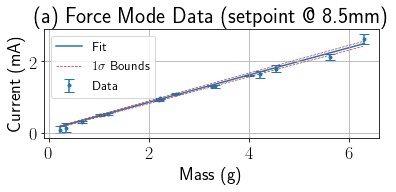
\includegraphics[width=0.95\linewidth]{figs/data/force_data.png}
    %\caption{Force data TODO}
    %\label{fig:force-data}
%\end{figure}

%\begin{figure}[t]
    %\centering
    %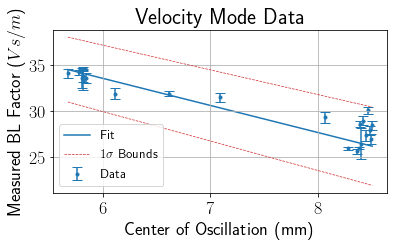
\includegraphics[width=0.95\linewidth]{figs/data/velocity_data.png}
    %\caption{Velocity data TODO}
    %\label{fig:velocity-data}
%\end{figure}





%\begin{center}
    %\begin{tabular}{|c|c|c|}\hline
        %Force Mode & Velocity Mode & Ratio \\\hline
        %25.1 & 25.6 & 1.02 \\\hline
    %\end{tabular}
    %\caption{$\Phi_B L$ factor measurements}
    %\label{tab:force_data}
%\end{center}


%\begin{table}[b]
    %\centering
    %\begin{tabular}{|c|c|c|}\hline
        %Force Mode & Velocity Mode & Ratio \\\hline
        %25.1 & 25.6 & 1.02 \\\hline
    %\end{tabular}
    %\caption{$\Phi_B L$ factor measurements}
    %\label{tab:force_data}
%\end{table}



%\begin{table}[h!]
%\centering
%\begin{tabular}{||c c c c||} 
 %\hline
 %Col1 & Col2 & Col2 & Col3 \\ [0.5ex] 
 %\hline\hline
 %1 & 6 & 87837 & 787 \\ 
 %2 & 7 & 78 & 5415 \\
 %3 & 545 & 778 & 7507 \\
 %4 & 545 & 18744 & 7560 \\
 %5 & 88 & 788 & 6344 \\ [1ex] 
 %\hline
%\end{tabular}
%\caption{Table to test captions and labels}
%\label{table:1}
%\end{table}
% \begin{figure}[h]
%     \centering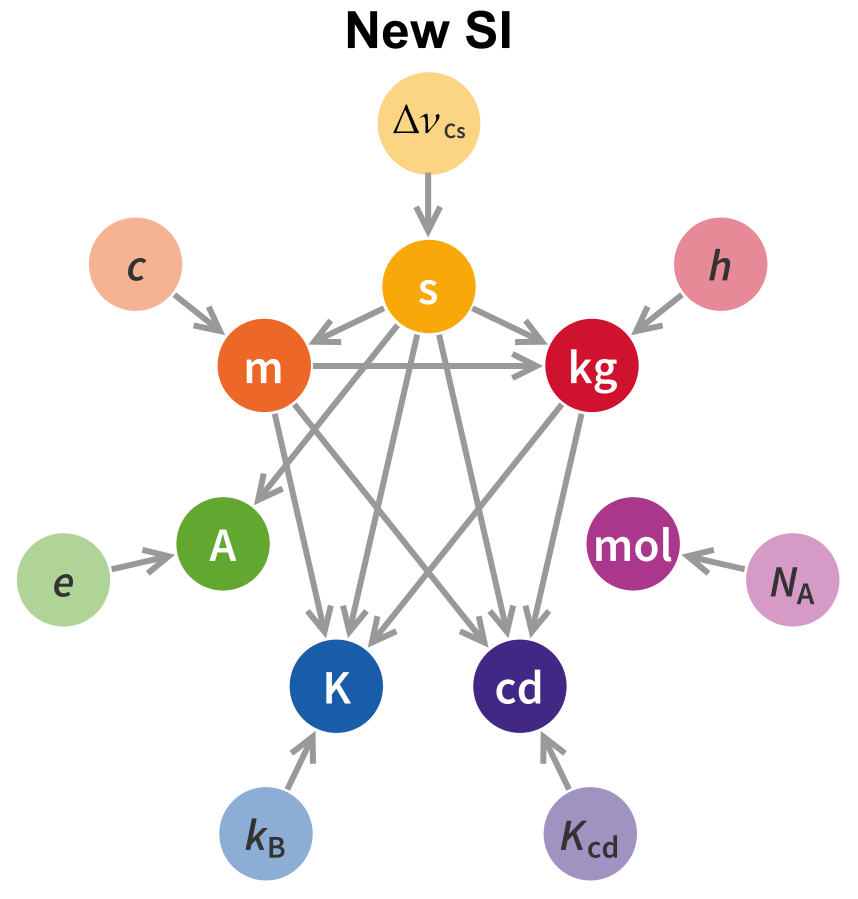
\includegraphics[width=.95\linewidth]{figs/si_units.png}
%     \caption{As of May 20, 2019, all SI units will be defined in terms of fundamental constants of the universe. 
%     % Notably, the units of kilogram, ampere, kelvin, and mole will be redefined in terms of Planck's constant $h$, the charge of an electron $e$, the Boltzmann constant $k$, and Avogagro's number $N_A$.
%     \cite{wiki_si}}\label{fig:si}
% \end{figure}

\section{CONCLUSION}

A Watt balance was built to measure the relationship between mechanical power and electrical power. Such a device could be used to measure the relationship between Planck's constant and the kilogram by using Josephson junctions and quantum resistance standards to measure electrical units in the experiment. The goal of the experiment was to measure unity in $\Phi_f/\Phi_v$, which was measured to be $0.98 \pm 0.11$.


 

% \newpage
% \nocite{lab_manual}
% \section{References}


\appendix
\newpage
    \section{Cross-Correlation}\label{apx:correlation}
    In signal processing, cross-correlation is equivalent to the convolution of two signals. The convolution of two discrete signals $f$ and $g$ is defined as
    \begin{equation}
        (f*g)[n] = \sum\limits_{m=-\infty}^\infty f[m]\ g[n-m]
        \label{eq:convolution}
    \end{equation}
    Figure~\ref{fig:correlation_example} illustrates an example of cross-correlation using two phase shifted sine signals. In figure~\ref{fig:correlation_example}a we see two sinusoidal signals, the second having a phase shift of $\pi/8$. Figure~\ref{fig:correlation_example}b shows the output of the cross-correlation function. The maximum correlation appears at $x\approx0.12\pi$. Shifting the data by this amount puts the signals in phase, as shown in figure~\ref{fig:correlation_example}c. 

    \begin{figure}[t]
        \centering
        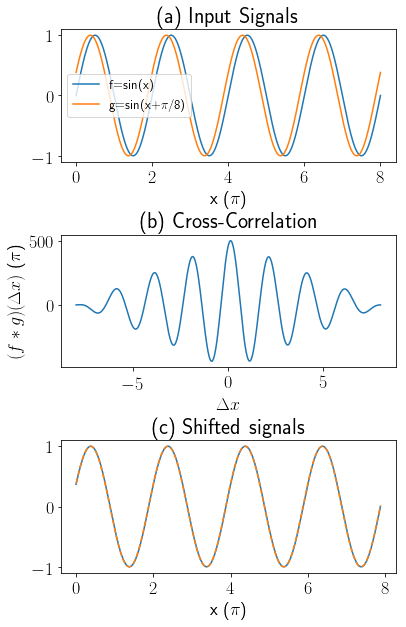
\includegraphics[width=0.95\linewidth]{figs/data/correlation_example.png}
        \caption{Cross-correlation example TODO}
        \label{fig:correlation_example}
    \end{figure}



% \onecolumngrid
% \newpage
% \begin{appendices}

% \section{Spectrum Analyzer 14.1.1}\label{apx:block-diagram-14.1.1}

% \appendixpdf{Embedded Microprocessor}{1042_source.pdf}{apx:1042_verilog}
% \end{appendices}


\bibliography{sources}
\end{document}
